\newpage
\section{Logic}

\subsection{Block definition diagram}
Blokdiagrammer giver et indblik på den overordnede strukturen af \textit{Konditioneringsapparatet}.  Hver kasse skal ses som en del der indgår i systemet \\
\begin{figure}[H]
	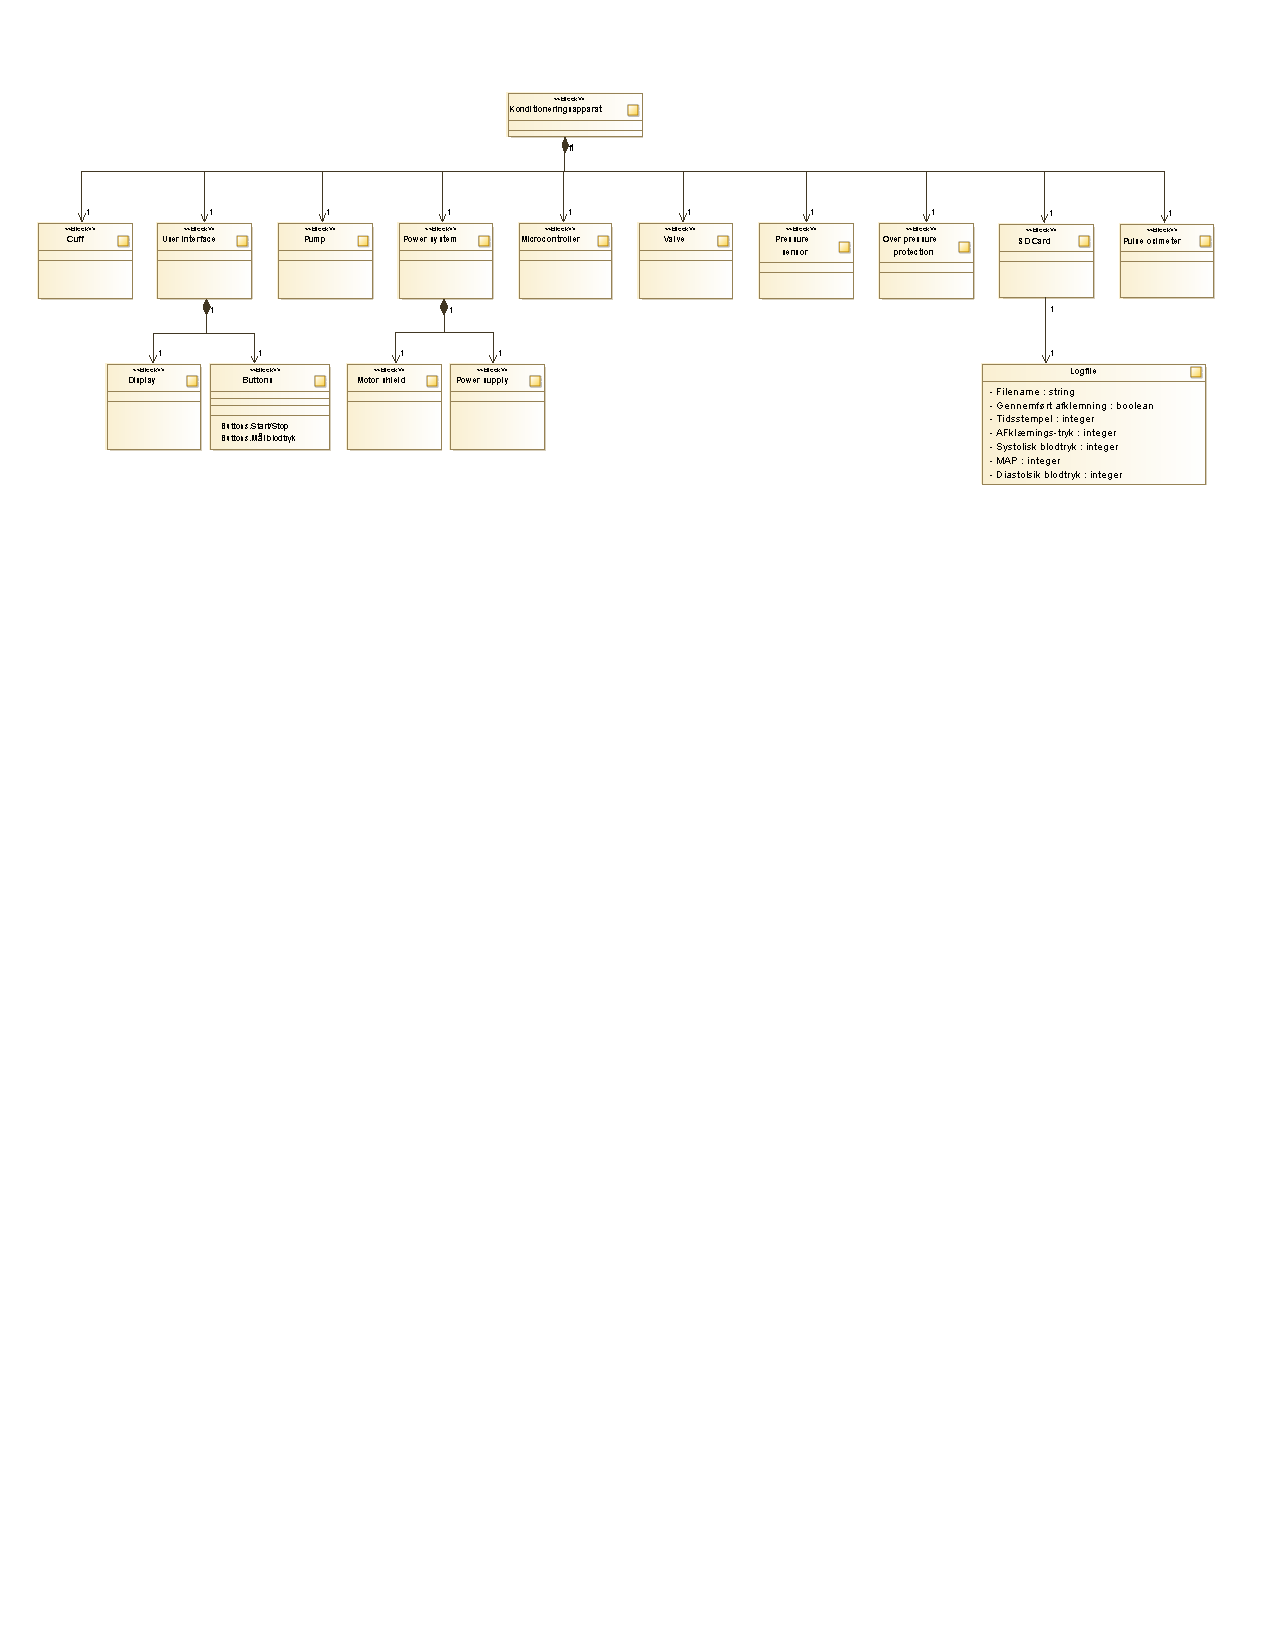
\includegraphics[width=\textwidth]{pdfs/BDD(SystemOverview).pdf}
	\caption{Block definition diagram over \textit{Konditioneringsapparatet}}
\end{figure}


\subsection{Domænemodel}
Diagrammer beskriver det systemet som helhed. Ved gennemgang af alle use cases findes væsentlig navneord og disse oprettet som konceptuelle klasser. Det konceptuelle klasser er derefter oversat til engelsk. \\
\begin{figure}[H]
	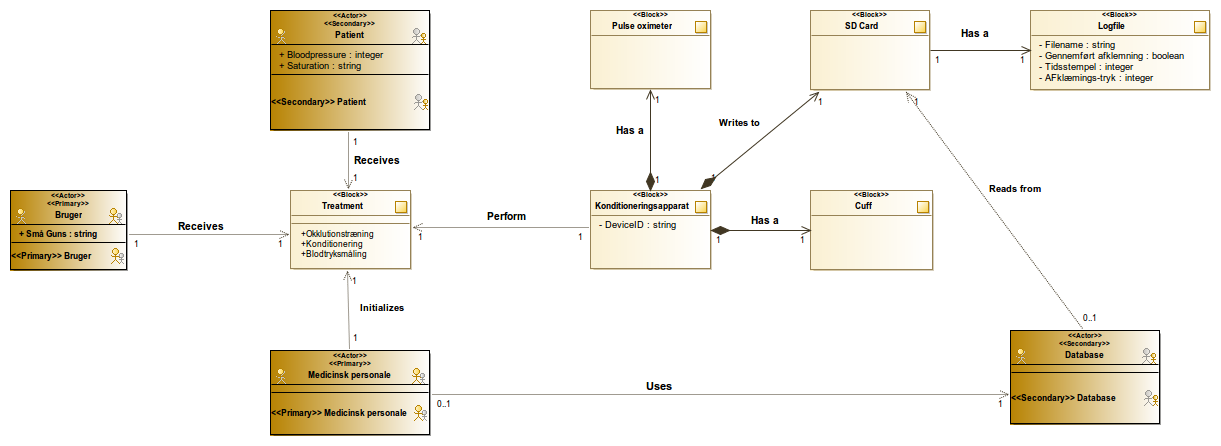
\includegraphics[width=\textwidth]{pdfs/DomainModel.png}
	\caption{Domæne model over \textit{Konditioneringsapparatet}}
\end{figure}


\newpage
\subsection{State machine diagram}
For at hjælpe med forståelsen af \textit{Konditioneringsapparatets} opbygning er der udarbejdet sekvens diagrammer over systemets tre programmer hhv. konditionering, okklusionstræning og setup. Der er desuden lavet et overordnede sekvens diagram over hele systemet. 
Sekvens diagrammerne beskæftiger sig med hvilke stadier programmet operer i, og hvilke parametre der skal være opfyldt før der skiftes til et andet stadie. 
 
\subsubsection{Boot}
\begin{figure}[H]
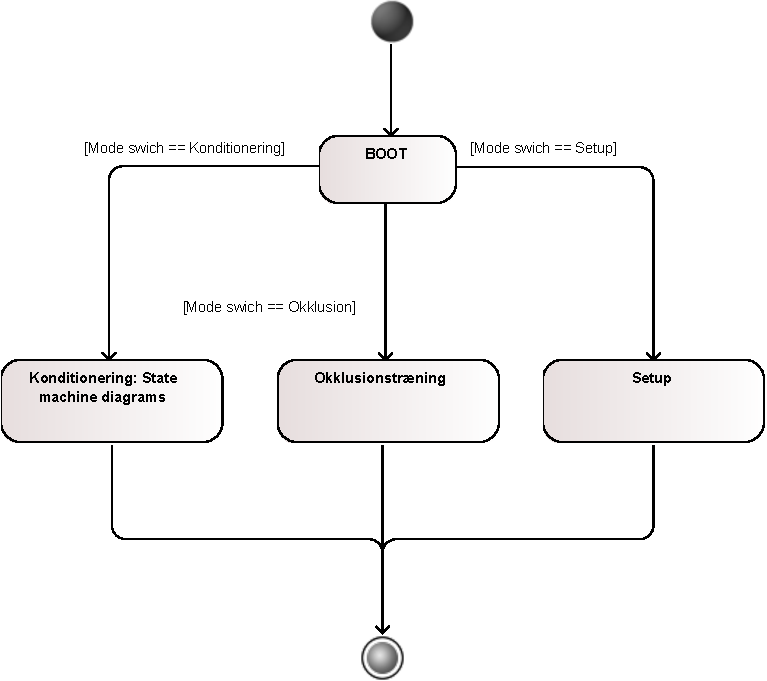
\includegraphics[width=\textwidth]{pdfs/STM_BOOT-crop.pdf} 
\caption{State machine diagram over programvalg på \textit{Konditioneringsapparatet}}
\end{figure}

\newpage
\subsubsection{Konditionering}
I programmet \textit{Konditionering} har brugeren mulighed for både at starte en konditioneringsbehandling eller måle et blodtryk, derfor er der udarbejdet et state machine diagram for hvert senarie. Beskrivelse af stadierne:
\begin{itemize}
	\item \textbf{Idle:} Stadie som programmet befinder sig i, før \textit{Medicinsk personale} har foretaget noget.
	\item \textbf{Deflate:} Reperfusionsfasen, efter en endt afklemning befinder systemets sig i denne fase.
	\item \textbf{Measure blood pressure:} Måling af blodtryk, ved knaptryk på [Start/Stop], efter en endt afklemningsfase eller hvis \textit{medicinsk personale} trykker på [Mål blodtryk].
	\item \textbf{Inflate:} Okklusionsstadiet, her befinder systemet sig hver gang en afklemning skal foretages.
\end{itemize}
Ved knaptryk på [Start/Stop] \\
\begin{figure}[H]
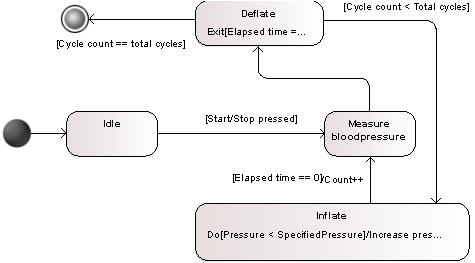
\includegraphics[width=\textwidth]{pdfs/STM_Konditionering1-crop.pdf}
\caption{State machine diagram over Konditioneringsforløb}
\end{figure}

Ved knaptryk på [Mål blodtryk] \\
\begin{figure}[H]
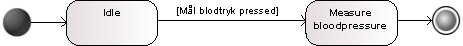
\includegraphics[width=\textwidth]{pdfs/STM_Konditionering2-crop.pdf}
\caption{State machine diagram over blodtryksmåling}
\end{figure}
\newpage

\subsubsection{Okklusion}
Beskrivelse af stadierne:
\begin{itemize}
	\item \textbf{Idle:} Stadie som programmet befinder sig i, før brugeren har foretaget noget.
	\item \textbf{Inflate:} Ved knaptryk på [Start/Stop] skifter systemet til dette stadie, her holdes trykket konstant på 100mmHg.
	\item \textbf{Deflate:} Dette stadie er manchetten tømt for luft.
\end{itemize}
	\begin{figure}[H]
		\begin{center}
		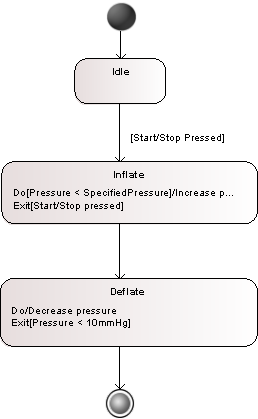
\includegraphics[width=0.5\textwidth]{pdfs/STM_Okklusion-crop.pdf}
		\caption{State machine diagram over okklusionsforløb}
	\end{center}
	\end{figure}

\newpage

\subsubsection{Setup}
Dette state machine diagram beskriver stadierne for programmet \textit{Setup}. Dette program har ingen slut stadie, cirklen med en cirklen inden i, da dette program ikke kan forlades, uden at apparatet slukkes. Beskrivels af stadier 
\begin{itemize}
	\item \textbf{Occlusiontime:} Stadie hvor \textit{Medicinsk personale} kan ændre tidsintervallet for hvor længe en afklemnings skal vare. 
	\item \textbf{Total number of cycles:} Opsætning af hvor mange afklemnings/reperfusions cyklusser systemet skal udføre. 
	\item \textbf{Selected} og \textbf{Change value:} er begge stadier hvor \textit{Medicinsk personale} enten skifter mellem \textit{Tid pr cyklus} og \textit{Antal cyklusser} eller ændringen af disse værdier.
	
\end{itemize}
\begin{figure}[H]
	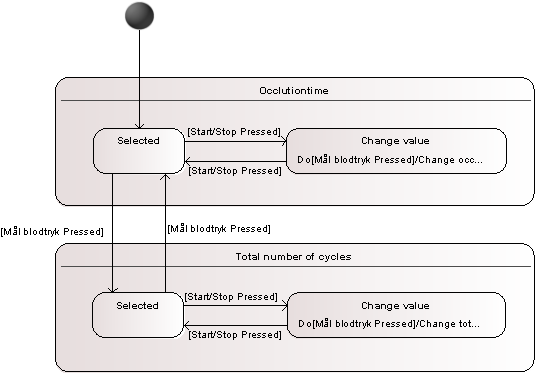
\includegraphics[width=\textwidth]{pdfs/STM_Setup-crop.pdf}
	\caption{State machine diagram over setup forløbet}
\end{figure}

